
% Default to the notebook output style

    


% Inherit from the specified cell style.




    
\documentclass[11pt,dvipdfmx]{jsarticle}

    
    
    \usepackage[T1]{fontenc}
    % Nicer default font (+ math font) than Computer Modern for most use cases
    \usepackage{mathpazo}

    % Basic figure setup, for now with no caption control since it's done
    % automatically by Pandoc (which extracts ![](path) syntax from Markdown).
   \usepackage{wrapfig}
    \usepackage{graphicx}
    % We will generate all images so they have a width \maxwidth. This means
    % that they will get their normal width if they fit onto the page, but
    % are scaled down if they would overflow the margins.
    \makeatletter
    \def\maxwidth{\ifdim\Gin@nat@width>\linewidth\linewidth
    \else\Gin@nat@width\fi}
    \makeatother
    \let\Oldincludegraphics\includegraphics
    % Set max figure width to be 80% of text width, for now hardcoded.
%    \renewcommand{\includegraphics}[1]{\Oldincludegraphics[width=.8\maxwidth]{#1}}
    % Ensure that by default, figures have no caption (until we provide a
    % proper Figure object with a Caption API and a way to capture that
    % in the conversion process - todo).
    \usepackage{caption}
%    \DeclareCaptionLabelFormat{nolabel}{}
%    \captionsetup{labelformat=nolabel}

    \usepackage{adjustbox} % Used to constrain images to a maximum size 
    \usepackage{xcolor} % Allow colors to be defined
    \usepackage{enumerate} % Needed for markdown enumerations to work
    \usepackage{geometry} % Used to adjust the document margins
    \usepackage{amsmath} % Equations
    \usepackage{amssymb} % Equations
    \usepackage{textcomp} % defines textquotesingle
    % Hack from http://tex.stackexchange.com/a/47451/13684:
    \AtBeginDocument{%
        \def\PYZsq{\textquotesingle}% Upright quotes in Pygmentized code
    }
    \usepackage{upquote} % Upright quotes for verbatim code
    \usepackage{eurosym} % defines \euro
    \usepackage[mathletters]{ucs} % Extended unicode (utf-8) support
    \usepackage[utf8x]{inputenc} % Allow utf-8 characters in the tex document
    \usepackage{fancyvrb} % verbatim replacement that allows latex
    \usepackage{grffile} % extends the file name processing of package graphics 
                         % to support a larger range 
    % The hyperref package gives us a pdf with properly built
    % internal navigation ('pdf bookmarks' for the table of contents,
    % internal cross-reference links, web links for URLs, etc.)
    \usepackage{hyperref}
    \usepackage{longtable} % longtable support required by pandoc >1.10
    \usepackage{booktabs}  % table support for pandoc > 1.12.2
    \usepackage[inline]{enumitem} % IRkernel/repr support (it uses the enumerate* environment)
    \usepackage[normalem]{ulem} % ulem is needed to support strikethroughs (\sout)
                                % normalem makes italics be italics, not underlines
    

    
    
    % Colors for the hyperref package
    \definecolor{urlcolor}{rgb}{0,.145,.698}
    \definecolor{linkcolor}{rgb}{.71,0.21,0.01}
    \definecolor{citecolor}{rgb}{.12,.54,.11}

    % ANSI colors
    \definecolor{ansi-black}{HTML}{3E424D}
    \definecolor{ansi-black-intense}{HTML}{282C36}
    \definecolor{ansi-red}{HTML}{E75C58}
    \definecolor{ansi-red-intense}{HTML}{B22B31}
    \definecolor{ansi-green}{HTML}{00A250}
    \definecolor{ansi-green-intense}{HTML}{007427}
    \definecolor{ansi-yellow}{HTML}{DDB62B}
    \definecolor{ansi-yellow-intense}{HTML}{B27D12}
    \definecolor{ansi-blue}{HTML}{208FFB}
    \definecolor{ansi-blue-intense}{HTML}{0065CA}
    \definecolor{ansi-magenta}{HTML}{D160C4}
    \definecolor{ansi-magenta-intense}{HTML}{A03196}
    \definecolor{ansi-cyan}{HTML}{60C6C8}
    \definecolor{ansi-cyan-intense}{HTML}{258F8F}
    \definecolor{ansi-white}{HTML}{C5C1B4}
    \definecolor{ansi-white-intense}{HTML}{A1A6B2}

    % commands and environments needed by pandoc snippets
    % extracted from the output of `pandoc -s`
    \providecommand{\tightlist}{%
      \setlength{\itemsep}{0pt}\setlength{\parskip}{0pt}}
    \DefineVerbatimEnvironment{Highlighting}{Verbatim}{commandchars=\\\{\}}
    % Add ',fontsize=\small' for more characters per line
    \newenvironment{Shaded}{}{}
    \newcommand{\KeywordTok}[1]{\textcolor[rgb]{0.00,0.44,0.13}{\textbf{{#1}}}}
    \newcommand{\DataTypeTok}[1]{\textcolor[rgb]{0.56,0.13,0.00}{{#1}}}
    \newcommand{\DecValTok}[1]{\textcolor[rgb]{0.25,0.63,0.44}{{#1}}}
    \newcommand{\BaseNTok}[1]{\textcolor[rgb]{0.25,0.63,0.44}{{#1}}}
    \newcommand{\FloatTok}[1]{\textcolor[rgb]{0.25,0.63,0.44}{{#1}}}
    \newcommand{\CharTok}[1]{\textcolor[rgb]{0.25,0.44,0.63}{{#1}}}
    \newcommand{\StringTok}[1]{\textcolor[rgb]{0.25,0.44,0.63}{{#1}}}
    \newcommand{\CommentTok}[1]{\textcolor[rgb]{0.38,0.63,0.69}{\textit{{#1}}}}
    \newcommand{\OtherTok}[1]{\textcolor[rgb]{0.00,0.44,0.13}{{#1}}}
    \newcommand{\AlertTok}[1]{\textcolor[rgb]{1.00,0.00,0.00}{\textbf{{#1}}}}
    \newcommand{\FunctionTok}[1]{\textcolor[rgb]{0.02,0.16,0.49}{{#1}}}
    \newcommand{\RegionMarkerTok}[1]{{#1}}
    \newcommand{\ErrorTok}[1]{\textcolor[rgb]{1.00,0.00,0.00}{\textbf{{#1}}}}
    \newcommand{\NormalTok}[1]{{#1}}
    
    % Additional commands for more recent versions of Pandoc
    \newcommand{\ConstantTok}[1]{\textcolor[rgb]{0.53,0.00,0.00}{{#1}}}
    \newcommand{\SpecialCharTok}[1]{\textcolor[rgb]{0.25,0.44,0.63}{{#1}}}
    \newcommand{\VerbatimStringTok}[1]{\textcolor[rgb]{0.25,0.44,0.63}{{#1}}}
    \newcommand{\SpecialStringTok}[1]{\textcolor[rgb]{0.73,0.40,0.53}{{#1}}}
    \newcommand{\ImportTok}[1]{{#1}}
    \newcommand{\DocumentationTok}[1]{\textcolor[rgb]{0.73,0.13,0.13}{\textit{{#1}}}}
    \newcommand{\AnnotationTok}[1]{\textcolor[rgb]{0.38,0.63,0.69}{\textbf{\textit{{#1}}}}}
    \newcommand{\CommentVarTok}[1]{\textcolor[rgb]{0.38,0.63,0.69}{\textbf{\textit{{#1}}}}}
    \newcommand{\VariableTok}[1]{\textcolor[rgb]{0.10,0.09,0.49}{{#1}}}
    \newcommand{\ControlFlowTok}[1]{\textcolor[rgb]{0.00,0.44,0.13}{\textbf{{#1}}}}
    \newcommand{\OperatorTok}[1]{\textcolor[rgb]{0.40,0.40,0.40}{{#1}}}
    \newcommand{\BuiltInTok}[1]{{#1}}
    \newcommand{\ExtensionTok}[1]{{#1}}
    \newcommand{\PreprocessorTok}[1]{\textcolor[rgb]{0.74,0.48,0.00}{{#1}}}
    \newcommand{\AttributeTok}[1]{\textcolor[rgb]{0.49,0.56,0.16}{{#1}}}
    \newcommand{\InformationTok}[1]{\textcolor[rgb]{0.38,0.63,0.69}{\textbf{\textit{{#1}}}}}
    \newcommand{\WarningTok}[1]{\textcolor[rgb]{0.38,0.63,0.69}{\textbf{\textit{{#1}}}}}
    
    
    % Define a nice break command that doesn't care if a line doesn't already
    % exist.
    \def\br{\hspace*{\fill} \\* }
    % Math Jax compatability definitions
    \def\gt{>}
    \def\lt{<}
    % Document parameters
    \title{final\_reserch}
    
    
    

    % Pygments definitions
    
\makeatletter
\def\PY@reset{\let\PY@it=\relax \let\PY@bf=\relax%
    \let\PY@ul=\relax \let\PY@tc=\relax%
    \let\PY@bc=\relax \let\PY@ff=\relax}
\def\PY@tok#1{\csname PY@tok@#1\endcsname}
\def\PY@toks#1+{\ifx\relax#1\empty\else%
    \PY@tok{#1}\expandafter\PY@toks\fi}
\def\PY@do#1{\PY@bc{\PY@tc{\PY@ul{%
    \PY@it{\PY@bf{\PY@ff{#1}}}}}}}
\def\PY#1#2{\PY@reset\PY@toks#1+\relax+\PY@do{#2}}

\expandafter\def\csname PY@tok@w\endcsname{\def\PY@tc##1{\textcolor[rgb]{0.73,0.73,0.73}{##1}}}
\expandafter\def\csname PY@tok@c\endcsname{\let\PY@it=\textit\def\PY@tc##1{\textcolor[rgb]{0.25,0.50,0.50}{##1}}}
\expandafter\def\csname PY@tok@cp\endcsname{\def\PY@tc##1{\textcolor[rgb]{0.74,0.48,0.00}{##1}}}
\expandafter\def\csname PY@tok@k\endcsname{\let\PY@bf=\textbf\def\PY@tc##1{\textcolor[rgb]{0.00,0.50,0.00}{##1}}}
\expandafter\def\csname PY@tok@kp\endcsname{\def\PY@tc##1{\textcolor[rgb]{0.00,0.50,0.00}{##1}}}
\expandafter\def\csname PY@tok@kt\endcsname{\def\PY@tc##1{\textcolor[rgb]{0.69,0.00,0.25}{##1}}}
\expandafter\def\csname PY@tok@o\endcsname{\def\PY@tc##1{\textcolor[rgb]{0.40,0.40,0.40}{##1}}}
\expandafter\def\csname PY@tok@ow\endcsname{\let\PY@bf=\textbf\def\PY@tc##1{\textcolor[rgb]{0.67,0.13,1.00}{##1}}}
\expandafter\def\csname PY@tok@nb\endcsname{\def\PY@tc##1{\textcolor[rgb]{0.00,0.50,0.00}{##1}}}
\expandafter\def\csname PY@tok@nf\endcsname{\def\PY@tc##1{\textcolor[rgb]{0.00,0.00,1.00}{##1}}}
\expandafter\def\csname PY@tok@nc\endcsname{\let\PY@bf=\textbf\def\PY@tc##1{\textcolor[rgb]{0.00,0.00,1.00}{##1}}}
\expandafter\def\csname PY@tok@nn\endcsname{\let\PY@bf=\textbf\def\PY@tc##1{\textcolor[rgb]{0.00,0.00,1.00}{##1}}}
\expandafter\def\csname PY@tok@ne\endcsname{\let\PY@bf=\textbf\def\PY@tc##1{\textcolor[rgb]{0.82,0.25,0.23}{##1}}}
\expandafter\def\csname PY@tok@nv\endcsname{\def\PY@tc##1{\textcolor[rgb]{0.10,0.09,0.49}{##1}}}
\expandafter\def\csname PY@tok@no\endcsname{\def\PY@tc##1{\textcolor[rgb]{0.53,0.00,0.00}{##1}}}
\expandafter\def\csname PY@tok@nl\endcsname{\def\PY@tc##1{\textcolor[rgb]{0.63,0.63,0.00}{##1}}}
\expandafter\def\csname PY@tok@ni\endcsname{\let\PY@bf=\textbf\def\PY@tc##1{\textcolor[rgb]{0.60,0.60,0.60}{##1}}}
\expandafter\def\csname PY@tok@na\endcsname{\def\PY@tc##1{\textcolor[rgb]{0.49,0.56,0.16}{##1}}}
\expandafter\def\csname PY@tok@nt\endcsname{\let\PY@bf=\textbf\def\PY@tc##1{\textcolor[rgb]{0.00,0.50,0.00}{##1}}}
\expandafter\def\csname PY@tok@nd\endcsname{\def\PY@tc##1{\textcolor[rgb]{0.67,0.13,1.00}{##1}}}
\expandafter\def\csname PY@tok@s\endcsname{\def\PY@tc##1{\textcolor[rgb]{0.73,0.13,0.13}{##1}}}
\expandafter\def\csname PY@tok@sd\endcsname{\let\PY@it=\textit\def\PY@tc##1{\textcolor[rgb]{0.73,0.13,0.13}{##1}}}
\expandafter\def\csname PY@tok@si\endcsname{\let\PY@bf=\textbf\def\PY@tc##1{\textcolor[rgb]{0.73,0.40,0.53}{##1}}}
\expandafter\def\csname PY@tok@se\endcsname{\let\PY@bf=\textbf\def\PY@tc##1{\textcolor[rgb]{0.73,0.40,0.13}{##1}}}
\expandafter\def\csname PY@tok@sr\endcsname{\def\PY@tc##1{\textcolor[rgb]{0.73,0.40,0.53}{##1}}}
\expandafter\def\csname PY@tok@ss\endcsname{\def\PY@tc##1{\textcolor[rgb]{0.10,0.09,0.49}{##1}}}
\expandafter\def\csname PY@tok@sx\endcsname{\def\PY@tc##1{\textcolor[rgb]{0.00,0.50,0.00}{##1}}}
\expandafter\def\csname PY@tok@m\endcsname{\def\PY@tc##1{\textcolor[rgb]{0.40,0.40,0.40}{##1}}}
\expandafter\def\csname PY@tok@gh\endcsname{\let\PY@bf=\textbf\def\PY@tc##1{\textcolor[rgb]{0.00,0.00,0.50}{##1}}}
\expandafter\def\csname PY@tok@gu\endcsname{\let\PY@bf=\textbf\def\PY@tc##1{\textcolor[rgb]{0.50,0.00,0.50}{##1}}}
\expandafter\def\csname PY@tok@gd\endcsname{\def\PY@tc##1{\textcolor[rgb]{0.63,0.00,0.00}{##1}}}
\expandafter\def\csname PY@tok@gi\endcsname{\def\PY@tc##1{\textcolor[rgb]{0.00,0.63,0.00}{##1}}}
\expandafter\def\csname PY@tok@gr\endcsname{\def\PY@tc##1{\textcolor[rgb]{1.00,0.00,0.00}{##1}}}
\expandafter\def\csname PY@tok@ge\endcsname{\let\PY@it=\textit}
\expandafter\def\csname PY@tok@gs\endcsname{\let\PY@bf=\textbf}
\expandafter\def\csname PY@tok@gp\endcsname{\let\PY@bf=\textbf\def\PY@tc##1{\textcolor[rgb]{0.00,0.00,0.50}{##1}}}
\expandafter\def\csname PY@tok@go\endcsname{\def\PY@tc##1{\textcolor[rgb]{0.53,0.53,0.53}{##1}}}
\expandafter\def\csname PY@tok@gt\endcsname{\def\PY@tc##1{\textcolor[rgb]{0.00,0.27,0.87}{##1}}}
\expandafter\def\csname PY@tok@err\endcsname{\def\PY@bc##1{\setlength{\fboxsep}{0pt}\fcolorbox[rgb]{1.00,0.00,0.00}{1,1,1}{\strut ##1}}}
\expandafter\def\csname PY@tok@kc\endcsname{\let\PY@bf=\textbf\def\PY@tc##1{\textcolor[rgb]{0.00,0.50,0.00}{##1}}}
\expandafter\def\csname PY@tok@kd\endcsname{\let\PY@bf=\textbf\def\PY@tc##1{\textcolor[rgb]{0.00,0.50,0.00}{##1}}}
\expandafter\def\csname PY@tok@kn\endcsname{\let\PY@bf=\textbf\def\PY@tc##1{\textcolor[rgb]{0.00,0.50,0.00}{##1}}}
\expandafter\def\csname PY@tok@kr\endcsname{\let\PY@bf=\textbf\def\PY@tc##1{\textcolor[rgb]{0.00,0.50,0.00}{##1}}}
\expandafter\def\csname PY@tok@bp\endcsname{\def\PY@tc##1{\textcolor[rgb]{0.00,0.50,0.00}{##1}}}
\expandafter\def\csname PY@tok@fm\endcsname{\def\PY@tc##1{\textcolor[rgb]{0.00,0.00,1.00}{##1}}}
\expandafter\def\csname PY@tok@vc\endcsname{\def\PY@tc##1{\textcolor[rgb]{0.10,0.09,0.49}{##1}}}
\expandafter\def\csname PY@tok@vg\endcsname{\def\PY@tc##1{\textcolor[rgb]{0.10,0.09,0.49}{##1}}}
\expandafter\def\csname PY@tok@vi\endcsname{\def\PY@tc##1{\textcolor[rgb]{0.10,0.09,0.49}{##1}}}
\expandafter\def\csname PY@tok@vm\endcsname{\def\PY@tc##1{\textcolor[rgb]{0.10,0.09,0.49}{##1}}}
\expandafter\def\csname PY@tok@sa\endcsname{\def\PY@tc##1{\textcolor[rgb]{0.73,0.13,0.13}{##1}}}
\expandafter\def\csname PY@tok@sb\endcsname{\def\PY@tc##1{\textcolor[rgb]{0.73,0.13,0.13}{##1}}}
\expandafter\def\csname PY@tok@sc\endcsname{\def\PY@tc##1{\textcolor[rgb]{0.73,0.13,0.13}{##1}}}
\expandafter\def\csname PY@tok@dl\endcsname{\def\PY@tc##1{\textcolor[rgb]{0.73,0.13,0.13}{##1}}}
\expandafter\def\csname PY@tok@s2\endcsname{\def\PY@tc##1{\textcolor[rgb]{0.73,0.13,0.13}{##1}}}
\expandafter\def\csname PY@tok@sh\endcsname{\def\PY@tc##1{\textcolor[rgb]{0.73,0.13,0.13}{##1}}}
\expandafter\def\csname PY@tok@s1\endcsname{\def\PY@tc##1{\textcolor[rgb]{0.73,0.13,0.13}{##1}}}
\expandafter\def\csname PY@tok@mb\endcsname{\def\PY@tc##1{\textcolor[rgb]{0.40,0.40,0.40}{##1}}}
\expandafter\def\csname PY@tok@mf\endcsname{\def\PY@tc##1{\textcolor[rgb]{0.40,0.40,0.40}{##1}}}
\expandafter\def\csname PY@tok@mh\endcsname{\def\PY@tc##1{\textcolor[rgb]{0.40,0.40,0.40}{##1}}}
\expandafter\def\csname PY@tok@mi\endcsname{\def\PY@tc##1{\textcolor[rgb]{0.40,0.40,0.40}{##1}}}
\expandafter\def\csname PY@tok@il\endcsname{\def\PY@tc##1{\textcolor[rgb]{0.40,0.40,0.40}{##1}}}
\expandafter\def\csname PY@tok@mo\endcsname{\def\PY@tc##1{\textcolor[rgb]{0.40,0.40,0.40}{##1}}}
\expandafter\def\csname PY@tok@ch\endcsname{\let\PY@it=\textit\def\PY@tc##1{\textcolor[rgb]{0.25,0.50,0.50}{##1}}}
\expandafter\def\csname PY@tok@cm\endcsname{\let\PY@it=\textit\def\PY@tc##1{\textcolor[rgb]{0.25,0.50,0.50}{##1}}}
\expandafter\def\csname PY@tok@cpf\endcsname{\let\PY@it=\textit\def\PY@tc##1{\textcolor[rgb]{0.25,0.50,0.50}{##1}}}
\expandafter\def\csname PY@tok@c1\endcsname{\let\PY@it=\textit\def\PY@tc##1{\textcolor[rgb]{0.25,0.50,0.50}{##1}}}
\expandafter\def\csname PY@tok@cs\endcsname{\let\PY@it=\textit\def\PY@tc##1{\textcolor[rgb]{0.25,0.50,0.50}{##1}}}

\def\PYZbs{\char`\\}
\def\PYZus{\char`\_}
\def\PYZob{\char`\{}
\def\PYZcb{\char`\}}
\def\PYZca{\char`\^}
\def\PYZam{\char`\&}
\def\PYZlt{\char`\<}
\def\PYZgt{\char`\>}
\def\PYZsh{\char`\#}
\def\PYZpc{\char`\%}
\def\PYZdl{\char`\$}
\def\PYZhy{\char`\-}
\def\PYZsq{\char`\'}
\def\PYZdq{\char`\"}
\def\PYZti{\char`\~}
% for compatibility with earlier versions
\def\PYZat{@}
\def\PYZlb{[}
\def\PYZrb{]}
\makeatother


    % Exact colors from NB
    \definecolor{incolor}{rgb}{0.0, 0.0, 0.5}
    \definecolor{outcolor}{rgb}{0.545, 0.0, 0.0}



    
    % Prevent overflowing lines due to hard-to-break entities
    \sloppy 
    % Setup hyperref package
    \hypersetup{
      breaklinks=true,  % so long urls are correctly broken across lines
      colorlinks=true,
      urlcolor=urlcolor,
      linkcolor=linkcolor,
      citecolor=citecolor,
      }
    % Slightly bigger margins than the latex defaults
    
    \geometry{verbose,tmargin=1in,bmargin=1in,lmargin=1in,rmargin=1in}
    
    

    \begin{document}
    
    
    \maketitle
    
    

    
    Table of Contents{}

{{1~~}はじめに}

{{1.1~~}研究の目的}

{{1.2~~}研究の動機}

{{2~~}基本的事項}

{{2.1~~}Emacs}

{{2.2~~}Ruby}

{{2.3~~}RubyGems}

{{2.4~~}Keybind}

{{2.5~~}CUI(Character User Interface)}

{{2.6~~}使用したgemファイル}

{{2.6.1~~}diff-lcs}

{{2.6.2~~}Thor}

{{2.6.3~~}Minitest}

{{2.6.4~~}FileUtils}

{{2.6.5~~}open3}

{{2.6.6~~}Bundler}

{{2.6.7~~}Rubocop}

{{3~~}editor\_learnerの概要}

{{3.1~~}Installation}

{{3.1.1~~}githubによるinstall}

{{3.1.2~~}gemによるinstall}

{{3.2~~}uninstall}

{{3.2.1~~}githubからinstallした場合のuninstall方法}

{{3.2.2~~}gemからinstallした場合のuninstall方法}

{{3.3~~}動作環境}

{{3.3.1~~}error時の対処法}

{{3.4~~}初期設定}

{{3.5~~}delete}

{{3.6~~}random\_h.rbとsequential\_h.rb}

{{3.7~~}random\_checkの動作}

{{3.8~~}sequential\_checkの動作}

{{4~~}実装コードの解説}

{{4.1~~}起動時に毎回動作するプログラム}

{{4.1.1~~}プログラム内のインスタンス変数の概要}

{{4.1.2~~}Fileの作成}

{{4.2~~}ファイル削除処理delete}

{{4.3~~}random\_check}

{{4.4~~}sequential\_check}

{{4.4.1~~}インスタンス定数に格納されたパス}

{{4.4.2~~}動作部分}

{{4.5~~}新しいターミナルを開くopen\_terminal}

{{5~~}他のソフトとの比較}

{{5.1~~}PTYPING}

{{5.2~~}e-typing}

{{5.3~~}寿司打}

{{5.4~~}考察}

{{6~~}総括}

{{7~~}謝辞}

{{8~~}付録}

{{9~~}参考文献}

    \section{はじめに}\label{ux306fux3058ux3081ux306b}

    \subsection{研究の目的}\label{ux7814ux7a76ux306eux76eeux7684}

    editor\_learnerの開発の大きな目的はeditor(Emacs)操作,CUI操作(キーバインドなど),Ruby言語の習熟とタイピング速度の向上である.editor上で動かすためファイルの開閉,保存,画面分割といった基本操作を習熟することができ,Ruby言語のプログラムを写経することでRuby言語の習熟へと繋げる.更にコードを打つことで正しい運指を身につけタイピング速度の向上も図っている.コードを打つ際にキーバインドを利用することでGUIではなくCUI操作にも適応していく.これら全てはプログラマにとって作業を効率化させるだけでなく,プログラマとしての質の向上につながる.

    \subsection{研究の動機}\label{ux7814ux7a76ux306eux52d5ux6a5f}

    初めはタッチタイピングを習得した経験を活かして,西谷によって開発されたshunkuntype(ターミナル上で実行するタイピングソフト)の再開発をテーマにしていたが,これ以上タイピングに特化したソフトを開発しても同じようなものがWeb上に大量に転がっており,そのようなものをいくつも開発しても意味がないと考えた.そこで西谷研究室ではタイピング,Ruby言語,Emacsによるeditor操作,CUI操作の習熟が作業効率に非常に大きな影響を与えるので習熟を勧めている.そこで西谷研究室で使用されているeditorであるEmacs操作,Ruby言語の学習,タイピング速度,正確性の向上,CUI操作.これらの習熟を目的としたソフトを開発しようと考えた.

    \section{基本的事項}\label{ux57faux672cux7684ux4e8bux9805}

    \subsection{Emacs}\label{emacs}

    本研究において使用するeditorはEmacsである.ツールはプログラマ自身の手の延長である.これは他のどのようなソフトウェアツールよりもEditorに対して当てはまる.テキストはプログラミングにおける最も基本的な生素材なので,できる限り簡単に操作できる必要があります.

そこで西谷研究室で勧められているEmacsの機能については以下の通りである,

\begin{enumerate}
\def\labelenumi{\arabic{enumi}.}
\tightlist
\item
  設定可能である. フォント,色,ウィンドウサイズ,キーバインドを含めた全ての外見が好みに応じて設定できるようになっていること.通常の操作がキーストロークだけで行えると,手をキーボードから離す必要がなくなり,結果的にマウスやメニュー駆動型のコマンドよりも効率的に操作できるようになります
\item
  拡張性がある. 新しいプログラミング言語が出てきただけで,使い物にならなくなるようなエディタではなく,どんな新しい言語やテキスト形式が出てきたとしても,その言語の意味合いを「教え込む」ことが可能です
\item
  プログラム可能であること. 込み入った複数の手順を実行できるよう,Editorはプログラム可能であることが必須である.
\end{enumerate}

これらの機能は本来エディタが持つべき基本的な機能である.これらに加えてEmacsは,

\begin{enumerate}
\def\labelenumi{\arabic{enumi}.}
\tightlist
\item
  構文のハイライト Rubyの構文にハイライトを入れたい場合はファイル名の後に.rbと入れることでRubyモードに切り替わり構文にハイライトを入れることが可能になる.
\item
  自動インデント. テキストを編集する際,改行時に自動的にスペースやタブなどを入力しインデント調整を行ってくれる.
\end{enumerate}

などのプログラミング言語に特化した特徴を備えています.強力なeditorを習熟することは生産性を高めることに他ならない.カーソルの移動にしても,1回のキー入力で単語単位,行単位,ブロック単位,関数単位でカーソルを移動させることができれば,一文字ずつ,あるいは一行ずつ繰り返してキー入力を行う場合とは効率が大きく変わってきます.Emacsはこれらの全ての機能を孕んでいてeditorとして非常に優秀である.よって本研究はEmacsをベースとして研究を進める.

    \subsection{Ruby}\label{ruby}

Rubyの基本的な説明は以下の通り,Rubyはまつもとゆきひろにより開発されたオブジェクト指向スクリプト言語であり,スクリプト言語が用いられてきた領域でのオブジェクト指向プログラミングを実現する言語である.

本研究はRuby言語を使用しています.大きな理由としては

\begin{itemize}
\tightlist
\item
  構文の自由度が高く,記述量が少なくて済む.
\item
  強力な標準ライブラリが備えられている.
\end{itemize}

Rubyは変数の型付けがないため,記述量を少なく済ませることができ,"gem"という形式で公開されているライブラリが豊富かつ強力なので本研究はRuby言語を使用しました.

    \subsection{RubyGems}\label{rubygems}

Rubygemの基本的な説明は以下の通り,RubyGemsは,Ruby言語用のパッケージ管理システムであり,Rubyのプログラムと("gem"と呼ばれる)ライブラリの配布用標準フォーマットを提供している.gemを容易に管理でき,gemを配布するサーバの機能も持つ.

本研究ではRubyGemsのgemを利用してファイル操作やパスの受け取りなどを行い,本研究で開発したソフトもgemに公開してある.

    \subsection{Keybind}\label{keybind}

Keybindの基本的な説明は以下の通り,押下するキー(単独キーまたは複数キーの組み合わせ)と,実行される機能との対応関係のことである.また,キーを押下したときに実行させる機能を割り当てる行為のことである.

以下controlを押しながらをc-と記述する.本研究におけるKeybindの習熟はCUI操作の習熟に酷似している.カーソル移動においてもGUIベースでマウスを使い行の先頭をクリックするより,CUIによりc-aを押すことで即座に行の先頭にカーソルを持っていくことができる.習熟するのであれば,どちらの方が早いかは一目瞭然である.本研究はKeybindの習熟によるCUI操作の適応で作業の効率化,高速化に重点を置いている.

    \subsection{CUI(Character User
Interface)}\label{cuicharacter-user-interface}

CUIは,キーボード等からの文字列を入力とし,文字列が表示されるウィンドウや古くはラインプリンタで印字される文字などを出力とする,ユーザインタフェースの様式で,GUI(Graphical
User Interface)の対義語として使われる.

CUIとGUIにはそれぞれ大きな違いがある.GUIの利点は以下の通り,

\begin{itemize}
\tightlist
\item
  文字だけでなくアイコンなどの絵も表示できる.
\item
  対象物が明確な点や,マウスで比較的簡単に操作できる.
\item
  即座に操作結果が反映される.
\end{itemize}

CUIの利点は以下の通り,

\begin{itemize}
\tightlist
\item
  コマンドを憶えていれば複雑な処理が簡単に行える.
\item
  キーボードから手を離すことなく作業の高速化が行える.
\end{itemize}

今回GUIではなくCUI操作の習熟を目的にした理由は,

\begin{itemize}
\tightlist
\item
  コマンドを憶えることで作業効率が上がる.
\item
  editor操作の習熟も孕んでいるから.
\end{itemize}

カーソル移動においてもGUIではなくCUI操作により,ワンコマンドで動かした方が効率的である.上記の理由から,GUIではなくCUI操作の習熟を目的としている.

    \subsection{使用したgemファイル}\label{ux4f7fux7528ux3057ux305fgemux30d5ux30a1ux30a4ux30eb}

    \subsubsection{diff-lcs}\label{diff-lcs}

    diff-lcsは,二つのファイルの差分を求めて出力してくれる.テキストの差分を取得するメソッドは,Diff::LCS.sdiff
と Diff::LCS.diff
の2つがある.複数行の文字列を比較した場合の2つのメソッドの違いは以下のとおり.

\begin{enumerate}
\def\labelenumi{\arabic{enumi}.}
\tightlist
\item
  Diff::LCS.sdiff

  \begin{enumerate}
  \def\labelenumii{\arabic{enumii}.}
  \tightlist
  \item
    比較結果を1文字ずつ表示する
  \end{enumerate}
\item
  Diff::LCS.diff

  \begin{enumerate}
  \def\labelenumii{\arabic{enumii}.}
  \tightlist
  \item
    比較した結果,違いがあった行について,違いがあった箇所のみ表示する.
  \end{enumerate}
\end{enumerate}

今回使用したのは後者(Diff:LCS.diff)である.理由は間違った部分だけを表示した方が見やすいと考えたからである.

    \subsubsection{Thor}\label{thor}

    Thorは,コマンドラインツールの作成を支援するライブラリです.gitやbundlerのようなサブコマンドツールを簡単に作成することができます.
Thorの使用でサブコマンドを自然言語に近い形で覚えることができる.

    \subsubsection{Minitest}\label{minitest}

    Minitestはテストを自動化するためのテスト用のフレームワークである.Rubyにはいくつかのテスティングフレームワークがありますが,Minitestというフレームワークを利用した理由は以下の通りです.

\begin{enumerate}
\def\labelenumi{\arabic{enumi}.}
\tightlist
\item
  Rubyをインストールすると一緒にインストールされるため,特別なセットアップが不要.
\item
  学習コストが比較的低い.
\item
  Railsのデフォルトのテスティングフレームワークなので,Railsを開発するときにも知識を活かしやすい.
\end{enumerate}

上記の理由から,sequential\_checkではminitestを採用しております.

    \subsubsection{FileUtils}\label{fileutils}

    再帰的な削除などの基本的なファイル操作を行うためのライブラリ

    \subsubsection{open3}\label{open3}

    プログラムを実行し,そのプロセスの標準出力,標準入力,標準エラー出力にパイプをつなぐためのものである.

    \subsubsection{Bundler}\label{bundler}

Bundlerはアプリケーション谷で依存するgemパッケージを管理するためのツールです.1つのシステム上で複数のアプリケーションを開発する場合や,デプロイ時にアプリケーションに紐付けてgemパッケージを管理したい場合に利用される.

    \subsubsection{Rubocop}\label{rubocop}

RubocopはRubyのソースコード解析ツールである.Rubyスタイルガイドや他のスタイルガイドに準拠しているかどうかを自動チェックしてくれるソフトウェアです.自分が打ち込んだ問題文となるソースコードのチェックに使用しました.

    \section{editor\_learnerの概要}\label{editor_learnerux306eux6982ux8981}

    \subsection{Installation}\label{installation}

\subsubsection{githubによるinstall}\label{githubux306bux3088ux308binstall}

githubによるインストール方法は以下の通りである.

\begin{enumerate}
\def\labelenumi{\arabic{enumi}.}
\tightlist
\item
  "https://github.com/souki1103/editor\_learner" へアクセス
\item
  Clone or downloadを押下,SSHのURLをコピー
\item
  コマンドラインにてgit clone(コピーしたURL)を行う
\end{enumerate}

上記の手順で開発したファイルがそのまま自分のディレクトリにインストールされる.

\subsubsection{gemによるinstall}\label{gemux306bux3088ux308binstall}

gemによるインストール方法は以下の通りである.

\begin{enumerate}
\def\labelenumi{\arabic{enumi}.}
\tightlist
\item
  コマンドラインにてgem install editor\_learnerと入力,実行
\item
  ファイルがホームディレクトの.rbenv/versions/2.4.0/lib/ruby/gems/2.4.0/gemsにeditor\_learnerが収納される
\end{enumerate}

これでeditor\_learnerとコマンドラインで入力することで実行可能となる.

    \subsection{uninstall}\label{uninstall}

\subsubsection{githubからinstallした場合のuninstall方法}\label{githubux304bux3089installux3057ux305fux5834ux5408ux306euninstallux65b9ux6cd5}

gituhubからinstallした場合のuninstall方法は以下の通りである.

\begin{enumerate}
\def\labelenumi{\arabic{enumi}.}
\tightlist
\item
  ホームディレクトで

  \begin{enumerate}
  \def\labelenumii{\arabic{enumii}.}
  \tightlist
  \item
    rm -rf editor\_learnerを入力
  \end{enumerate}
\item
  ホームディレクトリからeditor\_learnerが削除されていることを確認する.
\end{enumerate}

以上がuninstall方法である.

\subsubsection{gemからinstallした場合のuninstall方法}\label{gemux304bux3089installux3057ux305fux5834ux5408ux306euninstallux65b9ux6cd5}

gemからinstallした場合のuninstall方法は以下の通りである.

\begin{enumerate}
\def\labelenumi{\arabic{enumi}.}
\tightlist
\item
  ターミナル上のコマンドラインで

  \begin{enumerate}
  \def\labelenumii{\arabic{enumii}.}
  \tightlist
  \item
    gem uninstall editor\_learnerを入力
  \end{enumerate}
\item
  ホームディレクトの.rbenv/versions/2.4.0/lib/ruby/gems/2.4.0/gemsにeditor\_learnerが削除されていることを確認する.
\end{enumerate}

以上がuninstall方法である.

    \subsection{動作環境}\label{ux52d5ux4f5cux74b0ux5883}

    Rubyのversionが2.4.0以上でなければ動かない.理由としては,gemに格納されているパスを正しいく受け渡しできないからである.2.4.0以下で動作させるためにはeditor\_learnerの最新versionのみを入れることによって動作することが確認できている.

\subsubsection{error時の対処法}\label{errorux6642ux306eux5bfeux51e6ux6cd5}

errorが出た場合は以下の方法を試してください

\begin{enumerate}
\def\labelenumi{\arabic{enumi}.}
\tightlist
\item
  rm -rf editor\_learnerをコマンドラインで入力
\end{enumerate}

これによりファイル生成によるバグを解消できる.もう一つの方法は

\begin{enumerate}
\def\labelenumi{\arabic{enumi}.}
\tightlist
\item
  gem uninstall editor\_learnerをコマンドラインで入力
\item
  全てのversionをuninstallする.
\item
  再度gem install editor\_learnerで最新versionのみをinstallする.
\end{enumerate}

上記の手順によりRubyのversionによるバグが解消されることが確認できている.現在起こるであろうと予想されるバグの解消法は上記の2つである.Rubyのversionが2.4.0以上であればなんの不具合もなく動作することが確認できている.

    \subsection{初期設定}\label{ux521dux671fux8a2dux5b9a}

    特別な初期設定はほとんどないが起動方法は以下の通りである,

\begin{enumerate}
\def\labelenumi{\arabic{enumi}.}
\tightlist
\item
  コマンドライン上にてeditor\_learnerを入力する.

  \begin{enumerate}
  \def\labelenumii{\arabic{enumii}.}
  \setcounter{enumii}{1}
  \tightlist
  \item
    editor\_learnerを起動することでホームディレクトリにeditor\_learner/workshopと呼ばれるファイルが作成される.workshopは作業場という意味である.
  \item
    workshopの中にquestion.rbとanswer.rb,random\_h.rbとruby\_1\textsubscript{ruby\_6が作成され,ruby\_1}ruby\_6の中に1.rb\textasciitilde{}3.rbが作成されていることを確認する.
  \end{enumerate}
\end{enumerate}

\begin{figure}[H]
\centering
\begin{center}
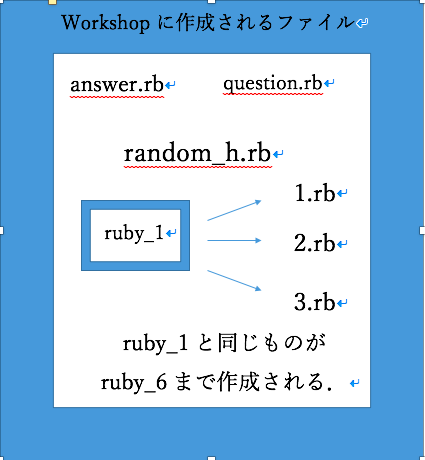
\includegraphics[width=150mm]{../../picture/mkdir.png}
\end{center}
\caption{File作られる画像.\label{sample}}

\label{fig:This}
\end{figure}

\begin{enumerate}
\def\labelenumi{\arabic{enumi}.}
\item
  起動すると以下のようなサブコマンドの書かれた画面が表示されることを確認する.

\begin{verbatim}
Commands:
editor_lerner delete [number~number]
editor_learner help [COMMAND]
editor_learner random_check
editor_leraner sequential_check [lesson_number] [1~3numbers]
\end{verbatim}
\item
  editor\_learnerの後にサブコマンドと必要に応じた引数を入力すると動作する.それぞれのサブコマンドの更に詳しい説明は以下の通りである.
\end{enumerate}

    \subsection{delete}\label{delete}

    editor\_learnerを起動することで初期設定で述べたようにホームディレクトリにeditor\_learner/workshopが作成される.deleteはworkshopに作成されたruby\_1\textasciitilde{}ruby\_6を削除するために作成されたものである.sequential\_checkで1度プログラムを作成してしまうと再度実行するとIt
have been
finished!と表示されてしまうので,削除するコマンドを作成しました.コマンド例は以下の通りである.

コマンド例

\begin{enumerate}
\def\labelenumi{\arabic{enumi}.}
\tightlist
\item
  editor\_learner delete 1 3
\end{enumerate}

上記のように入力することで1〜3までのファイルが削除される.サブコマンドの後の引数は2つの数字(char型)であり,削除するファイルの範囲を入力する.

    \subsection{random\_h.rbとsequential\_h.rb}\label{random_h.rbux3068sequential_h.rb}

random\_h.rbとsequential\_h.rbが初期設定で作成され,editor\_learnerを起動することで自動的に作成され,random\_checkとsequential\_checkを行う際に最初に開くファイルとなる.random\_check用とsequential\_check用に二つのファイルがある.random\_check用のファイルは以下の通りである.

random\_h.rb

\begin{figure}[H]
\centering
\begin{center}
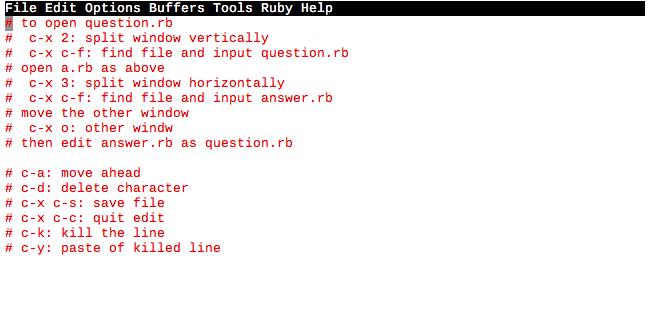
\includegraphics[width=150mm]{../../picture/random_h.png}
\end{center}
\caption{emacs の操作説明.\label{random_h}}

\label{fig:}
\end{figure}

上から順に説明すると, 1. question.rbを開くためにc-x
2で画面を2分割にする. 1. c-x c-fでquestion.rbを探して開く. 1.
次にanswer.rbを開くために画面を3分割する 1. 同様にc-x
c-fでanswer.rbを探して開く. 1. c-x
oでanswer.rbを編集するためにポインタを移動させる. 1.
question.rbに書かれているコードをanswer.rbに写す.

これらの手順がrandom\_h.rbに記述されている.全ての手順を終えたターミナルの状態は以下の通り,

\begin{figure}[H]
\centering
\begin{center}
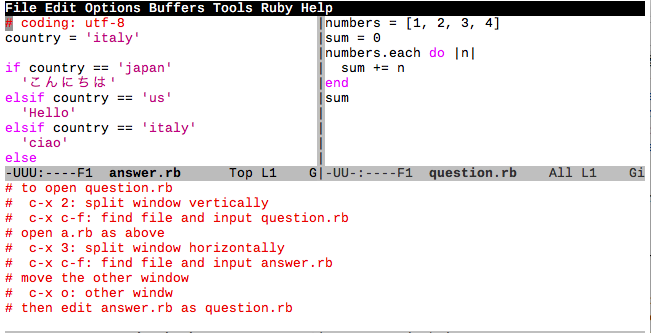
\includegraphics[width=150mm]{../../picture/split.png}
\end{center}
\caption{emacs の分割画面.\label{split}}

\label{fig:}
\end{figure}

上記の画像では,右上に問題であるquestion.rbが表示され,それを左上にあるanswer.rbに写す形となる.

次にsequential\_h.rb

\begin{figure}[H]
\centering
\begin{center}
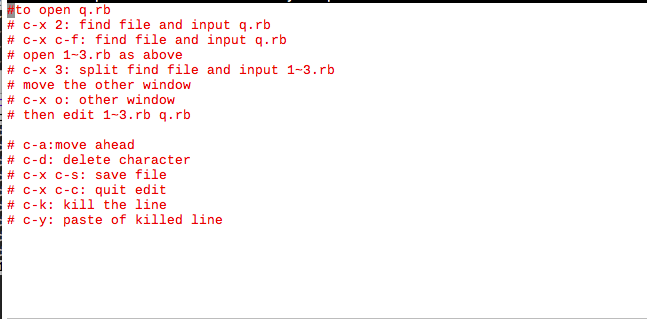
\includegraphics[width=150mm]{../../picture/sequential_h.png}
\end{center}
\caption{シーケンシャル.\label{sqquential}}

\label{fig:}
\end{figure}

書かれている内容自体はrandom\_h.rbとほとんど差異がないが,開くファイルの名前が違うため別のファイルとして作成された.この手順に沿って作業することになる.下に書かれているのは主要キーバインドであり,必要に応じて見て,使用する形となっている.上記の手順を行なったターミナル画面の状態はrandom\_h.rbの最終形態を同じである.

    \subsection{random\_checkの動作}\label{random_checkux306eux52d5ux4f5c}

random\_checkの動作開始から終了は以下の通りである.

\begin{enumerate}
\def\labelenumi{\arabic{enumi}.}
\tightlist
\item
  コマンドライン上にてeditor\_learne random\_checkを入力
\item
  新しいターミナル(ホームディレクトリ/editor\_learner/workshopから始まる)が開かれる.
\item
  random\_h.rbを開いてrandom\_h.rbに沿ってquestion.rbに書かれているコードをanswer.rbに写す.
\item
  前のターミナルに戻り,コマンドラインに"check"と入力することで正誤判定を行ってくれる.
\item
  間違っていればdiff-lcsにより間違った箇所が表示される.
\item
  正しければ新しいターミナルが開かれてから終了までの時間とIt have been
  finished!が表示され終了となる.
\end{enumerate}

更に次回random\_check起動時には前に書いたコードがanswer.rbに格納されたままなので全て削除するのではなく,前のコードの必要な部分は残すことができる.

random\_checkの大きな目的はtyping速度,正確性の向上,editor操作やRuby言語の習熟に重点を置いている.いかに早く終わらせるかのポイントがtyping速度,正確性とeditor操作である.

    \subsection{sequential\_checkの動作}\label{sequential_checkux306eux52d5ux4f5c}

    sequential\_checkの動作開始から終了は以下の通りである.

\begin{enumerate}
\def\labelenumi{\arabic{enumi}.}
\tightlist
\item
  コマンドライン上でeditor\_learner
  sequential\_check(1\textasciitilde{}6の数字)
  (1\textasciitilde{}3の数字)を入力
\item
  新しいターミナル(ホームディレクトリ/editor\_learner/workshop/ruby\_(1\textasciitilde{}6の数字))が開かれる.
\item
  sequential\_h.rbを開いてsequential\_h.rbに沿ってq.rbに書かれている内容を第2引数の数字.rbに写す.
\item
  前のターミナルに戻り,コマンドラインに"check"と入力することで正誤判定を行う.
\item
  間違っていれば間違った箇所が表示される.再度q.rbと第2引数の数字.rbを開いて間違った箇所を修正する.
\item
  正しければruby\_1/1.rb is done!のように表示される.
\end{enumerate}

sequential\_checkは1\textasciitilde{}3の順に1.rbがリファクタリングや追加され2.rbになり,完成形が3.rbになるといった形式である.連続的なプログラムの完成までを写経するのでsequential\_checkと名付けられた.

sequential\_checkの大きな目的はリファクタリングによるRuby言語の学習とCUI操作によるキーバインドの習熟,タイピング速度,正確性の向上に重点を置いている.コードがリファクタリングされる様を写経することで自分自身でRubyのコードを書くときに他の人が見やすくなるようなコードが書けるようになる.

    \section{実装コードの解説}\label{ux5b9fux88c5ux30b3ux30fcux30c9ux306eux89e3ux8aac}

本章では,今回作成したプログラムをライブラリ化し継続的な発展が可能なようにそれぞれの処理の解説を記述する.

    \subsection{起動時に毎回動作するプログラム}\label{ux8d77ux52d5ux6642ux306bux6bceux56deux52d5ux4f5cux3059ux308bux30d7ux30edux30b0ux30e9ux30e0}

editor\_learnerを起動したときに自動に動く部分である.コードは以下の通りである.

\begin{screen}
{\small
\begin{verbatim}
def initialize(*args)
      super
      @prac_dir="#{ENV['HOME']}/editor_learner/workshop"
      @lib_location = Open3.capture3("gem environment gemdir")
      @versions = Open3.capture3("gem list editor_learner")
      p @latest_version = @versions[0].chomp.gsub(' (', '-').gsub(')','')
      @inject = File.join(@lib_location[0].chomp, "/gems/#{@latest_version}/lib")
      if File.exist?(@prac_dir) != true then
        FileUtils.mkdir_p(@prac_dir)
        FileUtils.touch("#{@prac_dir}/question.rb")
        FileUtils.touch("#{@prac_dir}/answer.rb")
        FileUtils.touch("#{@prac_dir}/random_h.rb")
        if File.exist?("#{@inject}/random_h.rb") == true then
          FileUtils.cp("#{@inject}/random_h.rb", "#{@prac_dir}/random_h.rb")
        elsif
          FileUtils.cp("#{ENV['HOME']}/editor_learner/lib/random_h.rb", "#{@prac_dir}/random_h.rb")
        end
      end
      range = 1..6
      range_ruby = 1..3
      range.each do|num|
        if File.exist?("#{@prac_dir}/ruby_#{num}") != true then
          FileUtils.mkdir("#{@prac_dir}/ruby_#{num}")
          FileUtils.touch("#{@prac_dir}/ruby_#{num}/q.rb")
          FileUtils.touch("#{@prac_dir}/ruby_#{num}/sequential_h.rb")
          if File.exist?("#{@inject}/sequential_h.rb") == true then
            FileUtils.cp("#{@inject}/sequential_h.rb", "#{@prac_dir}/ruby_#{num}/sequential_h.rb")
          else
            FileUtils.cp("#{ENV['HOME']}/editor_learner/lib/sequential_h.rb", "#{@prac_dir}/ruby_#{num}/sequential_h.rb")
          end
          range_ruby.each do|n|
            FileUtils.touch("#{@prac_dir}/ruby_#{num}/#{n}.rb")
          end
        end
      end
    end
\end{verbatim}}
\end{screen}

この部分は基本的にディレクトリやファイルの作成が主である.上から順に説明すると,@prac\_dirはホームディレクトリ/editor\_learner/workshopを指しており,ファイルを作る際のパスとして作成されたインスタンス定数である.その後の3つのインスタンス定数(@lib\_location,@versions,@latest\_version)はgemでinstallされた場合ファイルの場所がホームディレクトリ/.rbenv/versions/2.4.0/lib/ruby/gems/2.4.0/gemsのeditor\_learnerに格納されているためgemでinstallした人とgithubでinstallした人とではパスが変わってしまうためこれらの3つのインスタンス定数を用意した.実際の振る舞いとしては,File.existによりprac\_dirがなければディレクトリを作成しさらにその中にquestion.rbとanswer.rbを作成する.gemにリリースしていることからgemでinstallした人とgithubでinstallした人のパスの違いをif文で条件分岐させている.これによりrandom\_h.rbを正常にコピーすることができた.

\subsubsection{プログラム内のインスタンス変数の概要}\label{ux30d7ux30edux30b0ux30e9ux30e0ux5185ux306eux30a4ux30f3ux30b9ux30bfux30f3ux30b9ux5909ux6570ux306eux6982ux8981}

インスタンス変数は,'@'で始まる変数はインスタンス変数であり,特定のオブジェクトに所属しています.インスタンス変数はそのクラスまたはサブクラスのメソッドから参照できます.初期化されない孫スタンス変数を参照した時の値はnillです.

このメソッドで使用されているインスタンス変数は5つである.prac\_dirはホームディレクトリ/editor\_learner/workshopを指しており,必要なファイルをここに作るのでパスとして受け渡すインスタンス変数となっている.その後の4つのインスタンス変数はgemからinstallした場合における,editor\_learnerが格納されているパスを受け渡すためのインスタンス変数である.一つずつの説明は以下の通り,

\begin{itemize}
\tightlist
\item
  lib\_locationはターミナル上で"gem environment
  gemdir"を入力した場合に出力されるパスを格納している.(自分のターミナル場で実行すると/Users/souki/.rbenv/versions/2.4.0/lib/ruby/gems/2.4.0)
\item
  versionsはgemでinstallされたeditor\_learnerのversionを受け取るためのパスを格納したインスタンス変数である.
\item
  latest\_versionははversionsで受け取ったeditor\_learnerのversionの最新部分のパスを格納したインスタンス変数である.
\item
  injectは実際にこれらのパスをつなぎ合わせてできるgemでinstallされたeditor\_learnerが格納されているパスが格納されているインスタン変数である.(自分の場合は/Users/souki/.rbenv/versions/2.4.0/lib/ruby/gems/2.4.0/gems/editor\_learner-1.1.2となる)
\end{itemize}

\subsubsection{Fileの作成}\label{fileux306eux4f5cux6210}

全てのパスの準備が整ったら実際に作業する場所に必要なファイル(question.rbやanswer.rb)などの作成が行われる.本研究のコードではeditor\_learner/workshopがホームディレクトリになければ作成する.さらに,その中にrandom\_checkに必要なファイル(question.rb,answer.rb,random\_h.rb)が作成される.random\_h.rbはgemでinstallした場合はeditor\_learnerの格納されている部分からコピーを行なっている.
次に,sequential\_checkに必要なファイルを作成する.editor\_learner/workshopにruby\_1\textsubscript{ruby6がなければ作成し,その中に1.rb}3.rbとq.rb(問題をコピーするためのファイル)とsequential\_h.rbが作成される.sequential\_h.rbはrandom\_h.rbと同じでgemからinstallした場合はeditor\_learnerの格納されている部分からコピーを行なっている.このメソッドの大きな役割はファイル作成である.

    \subsection{ファイル削除処理delete}\label{ux30d5ux30a1ux30a4ux30ebux524aux9664ux51e6ux7406delete}

sequential\_checkで終了したchapterをもう一度したい場合に一度ファイルを削除しなければいけないので,deleteメソッドの大きな役割はsequential\_checkで終了したファイルの削除である.

\begin{verbatim}
desc 'delete [number~number]', 'delete the ruby_file choose number to delet\
e file'

def delete(n, m)
  range = n..m
  range.each{|num|
  if File.exist?("#{@prac_dir}/ruby_#{num}") == true then
    system "rm -rf #{@prac_dir}/ruby_#{num}"
  end
  }
end
\end{verbatim}

コード自体はいたってシンプルで引数を2つ受け取ることでその間の範囲のFileを削除するようなコードとなっている.systemの"rm
-rf
ファイル名"がファイルを削除するコマンドなのでそこで受け取った引数の範囲でファイルの削除を行っている.

    \subsection{random\_check}\label{random_check}

random\_checkのコードは以下の通り,

\begin{verbatim}
desc 'random_check', 'ramdom check your typing and edit skill.'
    def random_check(*argv)
      random = rand(1..15)
      p random
      s = "#{random}.rb"
      puts "check starting ..."
      puts "type following commands on the terminal"
      puts "> emacs question.rb answer.rb"

      src_dir = File.expand_path('../..', __FILE__) # "Users/souki/editor_learner"
      if File.exist?("#{@inject}/random_check_question/#{s}") == true then
        FileUtils.cp("#{@inject}/random_check_question/#{s}", "#{@prac_dir}/question.rb")
      elsif
        FileUtils.cp(File.join(src_dir, "lib/random_check_question/#{s}"),  "#{@prac_dir}/question.rb")
      end
      open_terminal
      
      start_time = Time.now
      loop do
        a = STDIN.gets.chomp
        if a == "check" && FileUtils.compare_file("#{@prac_dir}/question.rb", "#{@prac_dir}/answer.rb") == true then
          puts "It have been finished!"
          break
        elsif FileUtils.compare_file("#{@prac_dir}/question.rb", "#{@prac_dir}/answer.rb") != true then
          @inputdata = File.open("#{@prac_dir}/answer.rb").readlines
          @checkdata = File.open("#{@prac_dir}/question.rb").readlines
          diffs = Diff::LCS.diff("#{@inputdata}", "#{@checkdata}")
          diffs.each do |diff|
            p diff
          end
        end
      end
      end_time = Time.now
      time = end_time - start_time - 1
      
      puts "#{time} sec"
    end
\end{verbatim}

random\_checkの概要を簡単に説明すると15個あるRubyのコードから1\textasciitilde{}15の乱数を取得し,選ばれた数字のファイルが問題としてコピーされて,それをanswer.rbに入力することで正解していたら新しいターミナルが開かれてから終了までの時間を評価する仕組みとなっている.

上から解説を行うと,1から15のrandomな乱数を取得,起動と同時にどのファイルがコピーされたか表示される.そして,src\_dirでホームディレクトリ/editor\_learnerのパスが代入される.そして,gemでinstallした人とgithubからcloneした場合によるファイルコピーのパスの違いをifで条件分岐.そして,1から15の乱数のファイルがquestion.rbにコピーされる.コピーされた後に新しいターミナルが開かれ,時間計測が開始される.そして,checkを前の画面に入力できるようにgetsを使った.初めにgetsだけを使用した時改行が入ってしまいうまく入力できなかった.しかし,chompを入れることで改行をなくすことに成功.しかし,argvとgetsを両方入れることが不可能なことが判明した.そこでgetsの前にSTDINを入れることでargvとの併用が可能なことがわかり,STDIN.gets.chompと入力することでキーボードからの入力を受け取ることができた.そして,checkが入力されてかつFileUtils.compareでファイルの比較で正しければ時間計測を終了し,表示する.間違っていた場合はインスタンス定数であるinputとoutputにquestion.rbとanswer.rbの中身が格納されてDiff::LCSのdiffによって間違っている箇所だけを表示する.一連のコード解説は以上である.

    \subsection{sequential\_check}\label{sequential_check}

sequential\_checkの場合はリファクタリングにあたりたくさんのインスタンス定数を作った.コードは以下の通り,

\begin{verbatim}
desc 'sequential_check [lesson_number] [1~3number] ','sequential check your typing skill and edit skill choose number'
    def sequential_check(*argv, n, m)
      l = m.to_i - 1
     
      @seq_dir = "lib/sequential_check_question"
      q_rb = "ruby_#{n}/#{m}.rb"
      @seqnm_dir = File.join(@seq_dir,q_rb)
      @pracnm_dir = "#{ENV['HOME']}/editor_learner/workshop/ruby_#{n}/#{m}.rb"
      @seqnq_dir = "lib/sequential_check_question/ruby_#{n}/q.rb"
      @pracnq_dir = "#{ENV['HOME']}/editor_learner/workshop/ruby_#{n}/q.rb"      
      @seqnl_dir = "lib/sequential_check_question/ruby_#{n}/#{l}.rb"
      @pracnl_dir = "#{ENV['HOME']}/editor_learner/workshop/ruby_#{n}/#{l}.rb"      
      puts "check starting ..."
      puts "type following commands on the terminal"
      src_dir = File.expand_path('../..', __FILE__)
      if File.exist?("#{@inject}/sequential_check_question/ruby_#{n}/#{m}.rb") == true then
        FileUtils.cp("#{@inject}/sequential_check_question/ruby_#{n}/#{m}.rb", "#{@pracnq_dir}")
      elsif
        FileUtils.cp(File.join(src_dir, "#{@seqnm_dir}"),  "#{@pracnq_dir}")
      end
      if l != 0 && FileUtils.compare_file("#{@pracnm_dir}", "#{@pracnq_dir}") != true
        FileUtils.compare_file("#{@pracnl_dir}", (File.join(src_dir, "#{@seqnl_dir}"))) == true
        FileUtils.cp("#{@pracnl_dir}", "#{@pracnm_dir}")
      end
      
      if FileUtils.compare_file(@pracnm_dir, @pracnq_dir) != true then
        system "osascript -e 'tell application \"Terminal\" to do script \"cd #{@prac_dir}/ruby_#{n} \" '"
        loop do
          a = STDIN.gets.chomp
          if a == "check" && FileUtils.compare_file("#{@pracnm_dir}", "#{@pracnq_dir}") == true then
            puts "ruby_#{n}/#{m}.rb is done!"
            break
          elsif FileUtils.compare_file("#{@pracnm_dir}", "#{@pracnq_dir}") != true then
            @inputdata = File.open("#{@pracnm_dir}").readlines
            @checkdata = File.open("#{@pracnq_dir}").readlines
            diffs = Diff::LCS.diff("#{@inputdata}", "#{@checkdata}")
            diffs.each do |diff|
              p diff
            end
          end
        end
       else
        p "ruby_#{n}/#{m}.rb is finished!"
      end
    end
\end{verbatim}

\subsubsection{インスタンス定数に格納されたパス}\label{ux30a4ux30f3ux30b9ux30bfux30f3ux30b9ux5b9aux6570ux306bux683cux7d0dux3055ux308cux305fux30d1ux30b9}

インスタンス定数に格納されているパスについての説明は上から順に以下の通り,

\begin{enumerate}
\def\labelenumi{\arabic{enumi}.}
\tightlist
\item
  seq\_dirはgithubでcloneした人が問題をコピーするときに使うパスである.
\item
  seqnm\_dirはその名の通りseq\_dirに引数であるnとmを代入したパスである.例として引数に1と1が代入された時は以下の通り,

  \begin{enumerate}
  \def\labelenumii{\arabic{enumii}.}
  \tightlist
  \item
    editor\_learner/sequential\_check\_question/ruby\_1/1.rbとなる.
  \end{enumerate}
\item
  pracnm\_dirはprac\_dirに二つの引数nとmを代入したものである.実際に作業するところのパスとして使用する.例として引数として1と1が代入された時は以下の通り,

  \begin{enumerate}
  \def\labelenumii{\arabic{enumii}.}
  \tightlist
  \item
    ホームディレクトリ/editor\_learner/workshop/ruby\_1/1.rbが格納される.
  \end{enumerate}
\item
  同様にseqとpracの後についている文字はその後のruby\_(数字)/(数字).rbの数字に入る文字を後につけている.
\end{enumerate}

\subsubsection{動作部分}\label{ux52d5ux4f5cux90e8ux5206}

まずgemでinstallした場合とgithubでinstallした場合による違いを条件分岐によりパスを変えている.さらに1.rbが終了していた場合2.rbに1.rbをコピーした状態から始まるように処理が行われている.その後は"check"が入力された時かつFileUtils.compareで正解していれば終了.間違っていればDiff::LCSで間違っている箇所を表示.もう一度修正し,"check"を入力,正解していれば終了.以上が一連のコードの解説である.

    \subsection{新しいターミナルを開くopen\_terminal}\label{ux65b0ux3057ux3044ux30bfux30fcux30dfux30caux30ebux3092ux958bux304fopen_terminal}

新しいターミナルを開くメソッドである.コードは以下の通りである.

\begin{verbatim}
def open_terminal
        pwd = Dir.pwd
        system "osascript -e 'tell application \"Terminal\" to do script \"cd #{@prac_dir} \" '"
      end
\end{verbatim}

新しく開かれたターミナルはprac\_dir(editor\_learner/workshop)のディレクトリからスタートするように設定されている.random\_checkではeditor\_learner/workshopでターミナルが開かれ,sequential\_checkではeditor\_learner/workshop/第1引数で入力されたファイルの場所が開かれるようになっている.

    \section{他のソフトとの比較}\label{ux4ed6ux306eux30bdux30d5ux30c8ux3068ux306eux6bd4ux8f03}

    他のタイピングソフトとの比較を行った表が以下の通りである.

\begin{figure}[H]
\centering
\begin{center}
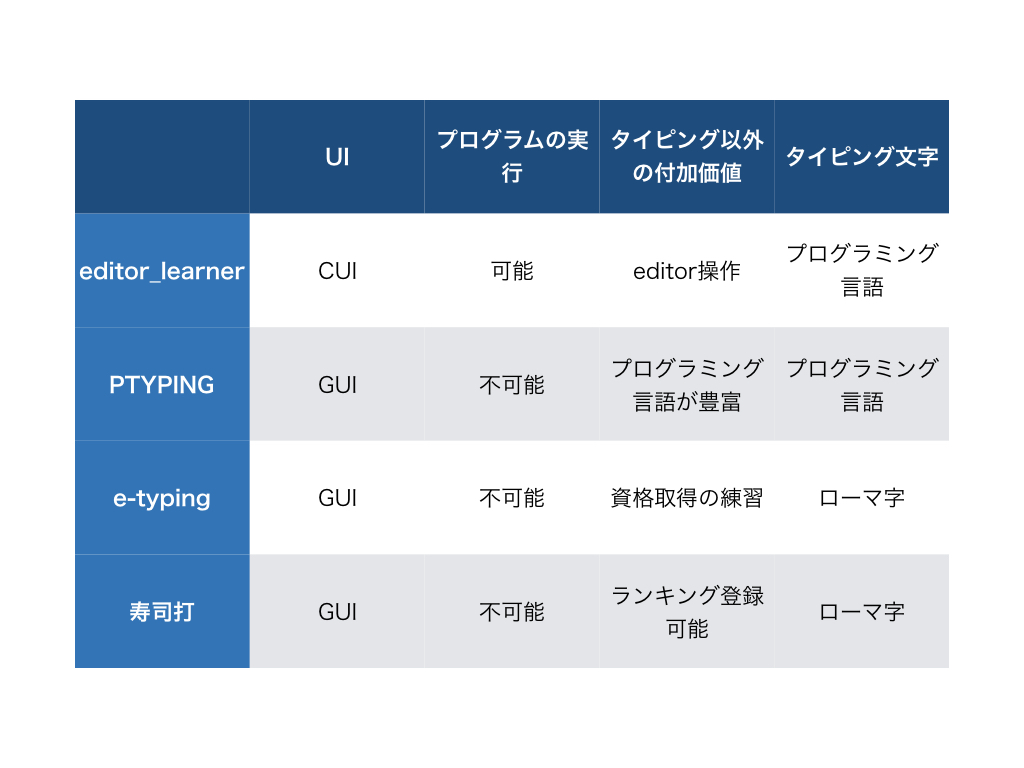
\includegraphics[width=150mm]{../../picture/compare.jpeg}
\end{center}
\caption{他のソフトとの比較.\label{compare}}

\label{fig:}
\end{figure}

上記のタイピングソフトは自分もよく使っていたタイピングソフトであり,評価も高いソフトである.それぞれの特徴は以下の通り,

\subsection{PTYPING}\label{ptyping}

PTYPINGは豊富なプログラム言語が入力可能である.しかし,コードを打つのではなく,コードに使われるintなどよく使われる単語が60秒の間にどれだけ打てるかというソフトです.

\subsection{e-typing}\label{e-typing}

e-typingはインターネットで無料提供されているソフトである.ローマ字入力を基本として,単語,短文,長文の3部構成となっておりタイピングの資格取得の練習もできる.

\subsection{寿司打}\label{ux5bffux53f8ux6253}

自分が一番利用したサイト,GUIベースによりローマ字入力を基本とし,打てば打つほど秒数が伸びていきどれだけ入力できるかをランキング形式で表示される.

\subsection{考察}\label{ux8003ux5bdf}

これら全てのソフトを利用した結果,editor\_learnerはローマ字入力ができない点では他のソフトに遅れをとるが,実際にプログラムを書くようになってからコードを写経することで\{\}や()などといったローマ字入力ではあまり入力しないような記号の入力が非常に早くなった.さらに,editor\_learnerは現段階ではRubyの学習のみだが,引数を変えて元となるプログラムを作成することで全てのプログラム言語を学ぶことができる.さらに,実際にコードを入力することができるソフトはたくさんあるが,実行可能なものは少ない(Webで行うものが大半を占めているから.)実際に西谷研究室でeditor\_learnerで学習を行っていない学生と行った自分のrandom\_check平均秒数は前者は200秒程なのに対して,自分は60秒程である.これらの結果からeditor\_learnerによる学習により,Ruby言語の学習にもなり,タイピング速度,正確性の向上,CUI操作の適応による差が出たと考えた.

    \section{総括}\label{ux7dcfux62ec}

    実際に今までたくさんのタイピングソフトやプログラムコードの打てるタイピングソフトを数多く利用してきたが,editor操作の習熟が可能なソフトは見たことも聞いたこともなかった.実際にタイピングだけが早い学生はたくさんいるがeditor操作やキーバインドも使いこなせる学生は少なかった.本研究で開発したeditor\_learnerによりそれらの技術も上達し,作業効率などの向上が見込める結果となった.

    \section{謝辞}\label{ux8b1dux8f9e}

    本研究を行うにあたり,終始多大なるご指導,御鞭撻をいただいた西谷滋人教授に対し,深く御礼申し上げます.また,本研究の進行に伴い,様々な助力,知識の供給をいただきました西谷研究室の同輩,先輩方に心から感謝の意を示します.本当にありがとうございました.

    \section{付録}\label{ux4ed8ux9332}

    \begin{verbatim}
require 'fileutils'
require 'colorize'
require 'thor'
require "editor_learner/version"
require 'diff-lcs'
require "open3"


module EditorLearner
class CLI < Thor

    def initialize(*args)
      super
      @prac_dir="#{ENV['HOME']}/editor_learner/workshop"
      @lib_location = Open3.capture3("gem environment gemdir")
      @versions = Open3.capture3("gem list editor_learner")
      p @latest_version = @versions[0].chomp.gsub(' (', '-').gsub(')','')
      @inject = File.join(@lib_location[0].chomp, "/gems/#{@latest_version}/lib")
      if File.exist?(@prac_dir) != true then
        FileUtils.mkdir_p(@prac_dir)
        FileUtils.touch("#{@prac_dir}/question.rb")
        FileUtils.touch("#{@prac_dir}/answer.rb")
        FileUtils.touch("#{@prac_dir}/random_h.rb")
        if File.exist?("#{@inject}/random_h.rb") == true then
          FileUtils.cp("#{@inject}/random_h.rb", "#{@prac_dir}/random_h.rb")
        elsif  
          FileUtils.cp("#{ENV['HOME']}/editor_learner/lib/random_h.rb", "#{@prac_dir}/random_h.rb")
        end
      end
      range = 1..6
      range_ruby = 1..3
      range.each do|num|
        if File.exist?("#{@prac_dir}/ruby_#{num}") != true then
          FileUtils.mkdir("#{@prac_dir}/ruby_#{num}")
          FileUtils.touch("#{@prac_dir}/ruby_#{num}/q.rb")
          FileUtils.touch("#{@prac_dir}/ruby_#{num}/sequential_h.rb")
          if File.exist?("#{@inject}/sequential_h.rb") == true then
            FileUtils.cp("#{@inject}/sequential_h.rb", "#{@prac_dir}/ruby_#{num}/sequential_h.rb")
          else
            FileUtils.cp("#{ENV['HOME']}/editor_learner/lib/sequential_h.rb", "#{@prac_dir}/ruby_#{num}/sequential_h.rb")
          end
          range_ruby.each do|n|
            FileUtils.touch("#{@prac_dir}/ruby_#{num}/#{n}.rb")
          end
        end
      end
    end
    
    desc 'delete [number~number]', 'delete the ruby_file choose number to delete file'
    
    def delete(n, m)
      range = n..m
      range.each{|num|
      if File.exist?("#{@prac_dir}/ruby_#{num}") == true then
        system "rm -rf #{@prac_dir}/ruby_#{num}"
      end
      }
    end

    desc 'sequential_check [lesson_number] [1~3number] ','sequential check your typing skill and edit skill choose number'
    def sequential_check(*argv, n, m)
      l = m.to_i - 1
     
      @seq_dir = "lib/sequential_check_question"
      q_rb = "ruby_#{n}/#{m}.rb"
      @seqnm_dir = File.join(@seq_dir,q_rb)
      @pracnm_dir = "#{ENV['HOME']}/editor_learner/workshop/ruby_#{n}/#{m}.rb"
      @seqnq_dir = "lib/sequential_check_question/ruby_#{n}/q.rb"
      @pracnq_dir = "#{ENV['HOME']}/editor_learner/workshop/ruby_#{n}/q.rb"      
      @seqnl_dir = "lib/sequential_check_question/ruby_#{n}/#{l}.rb"
      @pracnl_dir = "#{ENV['HOME']}/editor_learner/workshop/ruby_#{n}/#{l}.rb"      
      puts "check starting ..."
      puts "type following commands on the terminal"
      src_dir = File.expand_path('../..', __FILE__)
      if File.exist?("#{@inject}/sequential_check_question/ruby_#{n}/#{m}.rb") == true then
        FileUtils.cp("#{@inject}/sequential_check_question/ruby_#{n}/#{m}.rb", "#{@pracnq_dir}")
      elsif
        FileUtils.cp(File.join(src_dir, "#{@seqnm_dir}"),  "#{@pracnq_dir}")
      end
      if l != 0 && FileUtils.compare_file("#{@pracnm_dir}", "#{@pracnq_dir}") != true
        FileUtils.compare_file("#{@pracnl_dir}", (File.join(src_dir, "#{@seqnl_dir}"))) == true
        FileUtils.cp("#{@pracnl_dir}", "#{@pracnm_dir}")
      end
      
      if FileUtils.compare_file(@pracnm_dir, @pracnq_dir) != true then
        system "osascript -e 'tell application \"Terminal\" to do script \"cd #{@prac_dir}/ruby_#{n} \" '"
        loop do
          a = STDIN.gets.chomp
          if a == "check" && FileUtils.compare_file("#{@pracnm_dir}", "#{@pracnq_dir}") == true then
            puts "ruby_#{n}/#{m}.rb is done!"
            break
          elsif FileUtils.compare_file("#{@pracnm_dir}", "#{@pracnq_dir}") != true then
            @inputdata = File.open("#{@pracnm_dir}").readlines
            @checkdata = File.open("#{@pracnq_dir}").readlines
            diffs = Diff::LCS.diff("#{@inputdata}", "#{@checkdata}")
            diffs.each do |diff|
              p diff
            end
          end
        end
       else
        p "ruby_#{n}/#{m}.rb is finished!"
      end
    end

    desc 'random_check', 'ramdom check your typing and edit skill.'
    def random_check(*argv)
      random = rand(1..15)
      p random
      s = "#{random}.rb"
      puts "check starting ..."
      puts "type following commands on the terminal"
      puts "> emacs question.rb answer.rb"

      src_dir = File.expand_path('../..', __FILE__) # "Users/souki/editor_learner"
      if File.exist?("#{@inject}/random_check_question/#{s}") == true then
        FileUtils.cp("#{@inject}/random_check_question/#{s}", "#{@prac_dir}/question.rb")
      else
        FileUtils.cp(File.join(src_dir, "lib/random_check_question/#{s}"),  "#{@prac_dir}/question.rb")
      end
      open_terminal
      
      start_time = Time.now
      loop do
        a = STDIN.gets.chomp
        if a == "check" && FileUtils.compare_file("#{@prac_dir}/question.rb", "#{@prac_dir}/answer.rb") == true then
          puts "It have been finished!"
          break
        elsif FileUtils.compare_file("#{@prac_dir}/question.rb", "#{@prac_dir}/answer.rb") != true then
          @inputdata = File.open("#{@prac_dir}/answer.rb").readlines
          @checkdata = File.open("#{@prac_dir}/question.rb").readlines
          diffs = Diff::LCS.diff("#{@inputdata}", "#{@checkdata}")
          diffs.each do |diff|
            p diff
          end
        end
      end
      end_time = Time.now
      time = end_time - start_time - 1
      
      puts "#{time} sec"
    end
    
    no_commands do
      def open_terminal
        pwd = Dir.pwd
        system "osascript -e 'tell application \"Terminal\" to do script \"cd #{@prac_dir} \" '"
      end
    end
  end
end
\end{verbatim}

    \section{参考文献}\label{ux53c2ux8003ux6587ux732e}

    Andrew Hunt著,「達人プログラマー」 (オーム社出版,2016).


    % Add a bibliography block to the postdoc
    
    
    
    \end{document}
